%!TEX root = ../thesis.tex
%*******************************************************************************
%****************************** Second Chapter *********************************
%*******************************************************************************

\chapter{Experiments}
\label{chapter:experiments}

\graphicspath{{../img/plots/vae_latents/}{../img/plots/kodak_comparison/}{../img/plots/kodak_coding_time/}{../img/plots/kodak_side_info/}{../img/plots/reconstructions/}}

\label{sec:experimental_results}
\par
In this chapter, we detail our experimental setup and empirically show the
correctness and the efficiency of our model. We compare our results to
two classical lossy image compression methods, JPEG, and BPG. JPEG is the most
widely used lossy compression method (\cite{bull2014communicating}), and hence
showing that we can outperform it is important to show the viability of our
method. BPG (Better Portable Graphics) is a more modern transform coding method,
that adapts to the statistics of images and is the current state-of-the-art in
classical lossy image compression (\cite{rippel2017real}).
We also compare to the current state-of-the-art in neural compression, the results of
\cite{balle2018variational}\footnotemark. We implemented all of our
architectures and experiments from scratch in \texttt{Python 3.5}, using \texttt{Tensorflow}
(\cite{tensorflow2015-whitepaper}) and \texttt{Sonnet} (\cite{sonnetblog})
libraries. All of our code is available publicly at
\url{https://github.com/gergely-flamich/miracle-compression}. 

\footnotetext{We thank the authors of the paper for making their data available
  to us.}

\section{Experimental Setup}
\par
As we based our models on the work of \cite{balle2016end} and
\cite{balle2018variational}, we mirror a lot of their training setup as well
(see Section \ref{sec:dataset_preproc} for the dataset and preprocessing). We
trained all our models with Adam (\cite{kingma2014adam}) with a starting
learning rate of $\alpha_0 =
3 \times 10^{-5}$ and trained all of our models for 20 epochs or equivalently,
approximately 200,000 iterations, by using batches of 8 image patches per
iteration. For training VAEs and regular PLNs, we used a smooth
exponential learning rate decay schedule according to the formula
\[
  \alpha(t) = \alpha_0 \times r^{\frac{t}{D}}.
\]
Where $r$ is the decay rate, $D$ is the decay step size and $t$ is the current
iteration. We found $r = 0.96$ and $D = 1500$ worked well for our
experiments. While we did not notice significant performance gains using the
learning rate schedule, our models converged slightly faster.
\par
For $\gamma$-PLNs we found learning rate decay actually hurt the training
performance of the model, as it kept $\gamma$ from converging to 0.
\par
The architecture used for the VAE is the same as what we used for PLNs (shown in
Figure \ref{fig:pln_architecture}), with the second level omitted. For the
convolution capacities, we used $N = 192$ channels on the first
level and $M = 128$ channels on the second. We have significantly reduced the
channels on the latent dimensions compared to \cite{balle2018variational}, as we
use $F = 128$ and $G = 24$, where they use $F_{\text{Ball\'e}} = 192 / 320$, and
$G_{\text{Ball\'e}} = 128$. On the first level, we found that adding more
channels did not significantly increase the performance of our model, which we
credit to the more flexible latent distributions used in our model. On the other
hand, we chose $G = 24$ because we found that when increased beyond this, the
cost of communicating the group indices for the importance sampler became very
inefficient. With 24 channels, the overhead is already 30-40\% of the second
level's code length.
\par
In all experiments, we used the adaptive importance sampler on the second level and the
greedy sampler (IS-GS) on the first. For the importance sampler we used $K = 12$
bits as the outlier KL limit, $B = 20$ bits for the maximum total group KL and
$G = 16$ as the maximum number of dimensions in a single group. For the greedy
sampler, we set $K = 30$ shards and $B = 14$ bits per shard, leading to $2^{14}$
samples per shard. See Section \ref{sec:coded_sampling} for a review of these terms.

\paragraph{}
All experiments were run on a GeForce GTX 1080 GPU.

\section{Results}
\begin{figure}
  \centering
  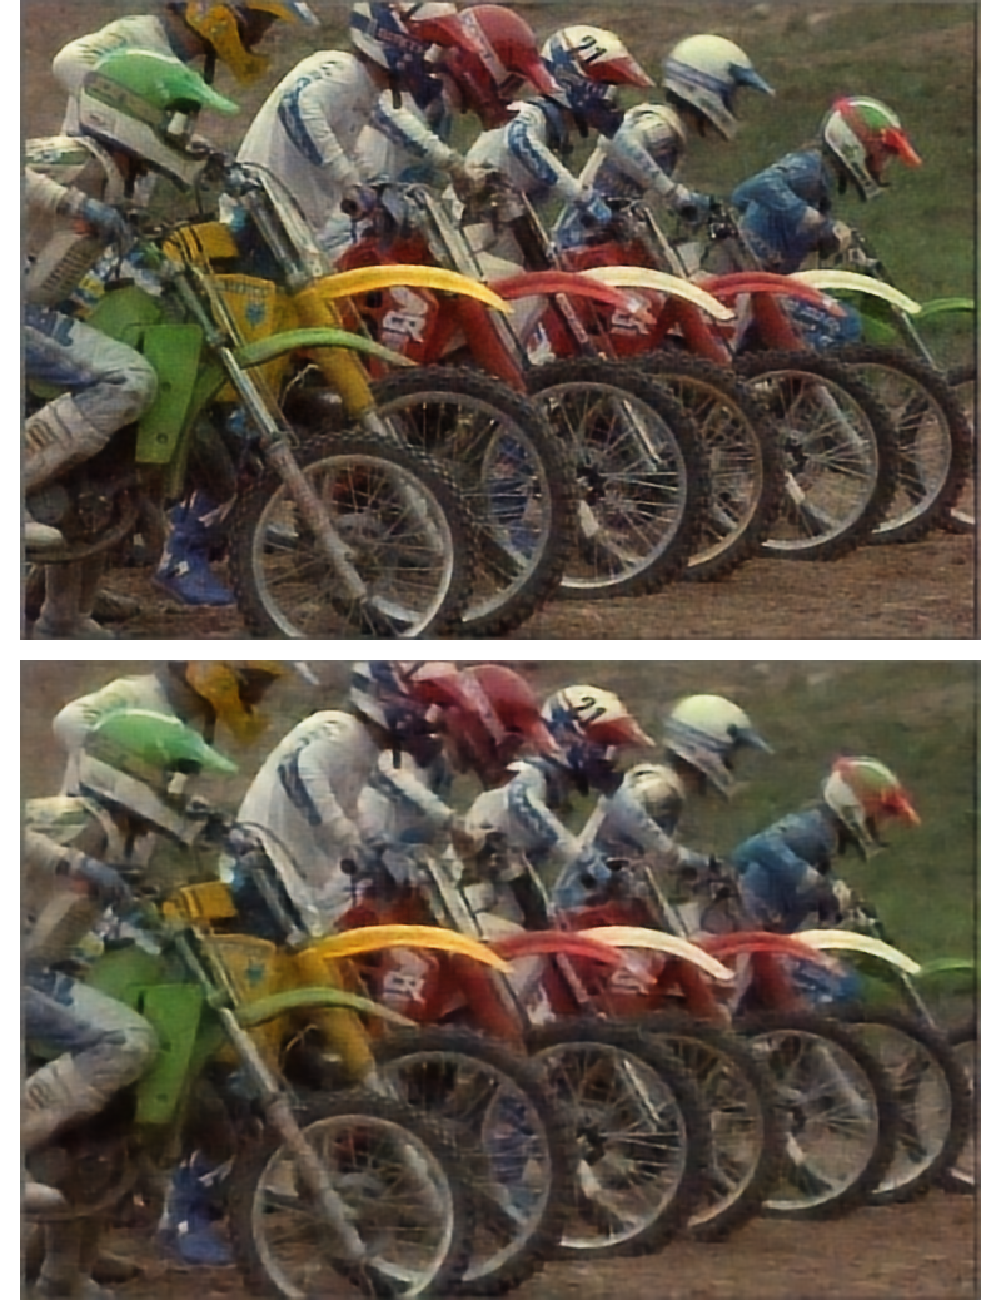
\includegraphics[width=\textwidth]{pln_003_01_k05.png}
  \caption[PLN reconstructions of \texttt{kodim05}.]
  {PLN reconstructions of \texttt{kodim05}. \textbf{Top:} $\beta =
    0.03$, 0.810 bpp, MS-SSIM: $0.913$, PSNR: $23.053$ dB \textbf{Bottom:}
    $\beta = 0.1$, 0.354 bpp, MS-SSIM: $0.848$, PSNR: $21.495$ dB.}
  \label{fig:pln_reconstruction}
\end{figure}
\begin{figure}
  \centering
  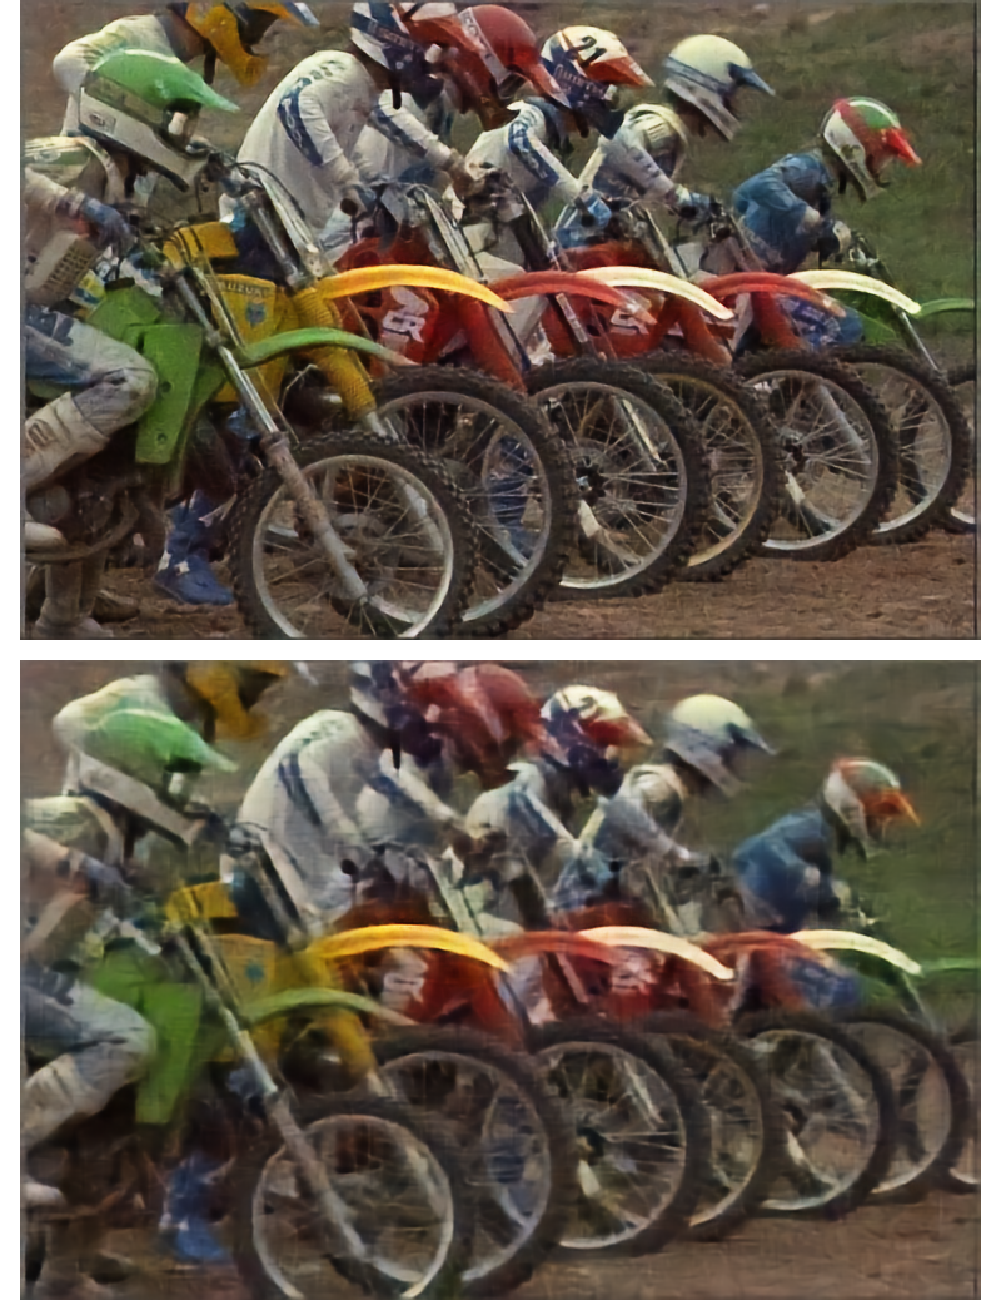
\includegraphics[width=\textwidth]{log_gamma_3_10_k05.png}
  \caption[$\gamma$-PLN reconstructions of \texttt{kodim05}.]
  {$\gamma$-PLN reconstructions of \texttt{kodim05}. \textbf{Top:}
    $\beta = 3$, 0.354 bpp, MS-SSIM: $0.937$, PSNR: $21.397$ dB \textbf{Bottom:}
    $\beta = 10$, 0.189 bpp, MS-SSIM: $0.824$, PSNR: $21.068$ dB.}
  \label{fig:gamma_reconstruction}
\end{figure}
\par

We present the rate-distortion curves for the following:
\begin{itemize}
\item JPEG, with quality settings from 1 to 92, with increments of 7 between
  settings. As this is the most widely used lossy image compression codec
  (\cite{bull2014communicating}), it is
  crucial to demonstrate that our method is at least competitive with it, and
  ideally beats it.
\item BPG\footnotemark with 4:4:4 chroma sampling, as we are comparing against
  RGB-based compression techniques. We used quantization settings between 51 to
  33 with decrements of 3 between settings.
\item Two models with the same architecture from \cite{balle2018variational},
  one optimized for an MSE training objective, and one optimized for the
  MS-SSIM perceptual metric.
\item Two of our models, all of which were optimized with Laplacian likelihoods,
  one PLN and one $\gamma$-PLN. We trained the PLNs using $\beta =
  \{1, 0.3, 0.1, 0.03\}$ and the $\gamma$-PLNs using $\beta =
  \{10, 3, 1, 0.3, 0.1\}$. We plot both their theoretically optimal
  performance as well as their actual performance, with the differences
  explained below. The reason for not presenting results of the VAEs is because
  their rate-distortion curves are quite a lot worse than the other
  models', and would have distorted the figures too much.
\end{itemize}

\par
When presenting our method, for each model we present two results: the \textit{theoretically
optimal} performance, and the \textit{actual} performance. The theoretically
optimal bits per pixel (BPP) was calculated using the theoretically
achievable upper bound for the compression size in bits as given by
Theorem \ref{thm:bits-back_efficiency}, without the constant term. Concretely,
for a drawn latent sample $\tilde{\vec{z}}$ for image $\vec{x}$, it is 
\[
  \KL{q_\phi(\vec{x} \mid \tilde{\vec{z}})}{p_\theta(\tilde{\vec{z}})}
  + 2 \log \left( \KL{q_\phi(\vec{x}
      \mid \tilde{\vec{z}})}{p_\theta(\tilde{\vec{z}})} + 1 \right).
\]
The optimal reconstruction error was calculated by passing an image through the
PLN using a normal forward pass, instead of using the IS-GS approximate sample. Thus, any
actual method's performance using the same setup should appear to the right of
(worse rate) or below (worse distortion) the theoretical position.

\footnotetext{We used the implementation available at \url{http://bellard.org/bpg}}

\par
We show a comparison between reconstructions at different rates of
\texttt{kodim05} from the Kodak Dataset (\cite{kodakdataset}) for PLNs in Figure
\ref{fig:pln_reconstruction} and for $\gamma$-PLNs in Figure
\ref{fig:gamma_reconstruction}. A much more thorough comparison of
reconstructions is given at the end of the thesis in Appendix \ref{chapter:appendix_b}.
\par
The rate-distortion curves for \texttt{kodim05} are shown in Figure
\ref{fig:kodim05_comp}. We observe a similar phenomenon as
\cite{balle2018variational}: there is a mismatch in the comparison
of models according to different perceptual metrics, depending on what objective
they have been optimized for. In particular, JPEG and BPG have both been
optimized so that they give high PSNR (thus, low MSE), whereas they underperform
on the newer MS-SSIM metric. MS-SSIM correlates better with how
the human visual system (HVS) perceives quality (\cite{msssim}),
hence it is generally more desirable to perform well on that metric
(\cite{toderici2017full}, \cite{rippel2017real}, \cite{balle2018variational}).
The fact that our models perform well on MS-SSIM also justifies our choice of
the MAE as the training objective.
\begin{figure}
  \centering
  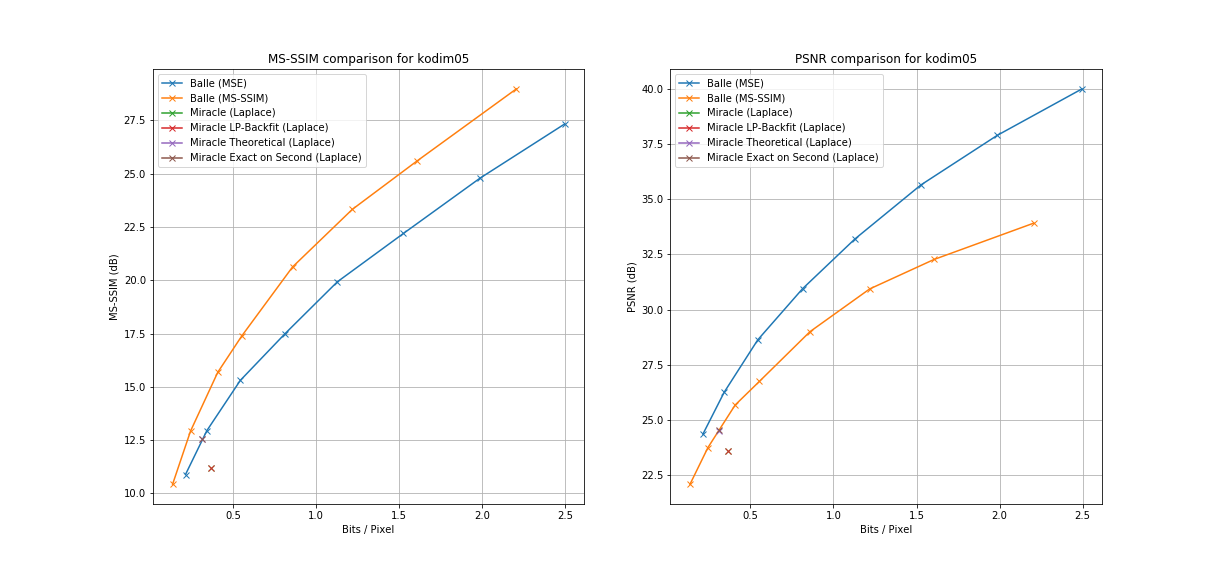
\includegraphics[width=\textwidth]{kodim05_comparison.png}
  \caption[Rate-Distorsion curves of several methods on \texttt{kodim05}]
  {Rate-Distorsion curves of several methods on \texttt{kodim05}. Please see
    Section \ref{sec:experimental_results} for the description of how we
    obtained each curve. MS-SSIM results are presented in
    decibels, where the conversion is done using the formula $-10 \cdot
    \log_{10}\left( 1 - \text{MS-SSIM}(\vec{x}, \hat{\vec{x}}) \right)$.
    PSNR is computed from the mean squared error, using the formula 
    $-10 \cdot \log_{10}\text{MSE}(\vec{x}, \hat{\vec{x}})$.}
  \label{fig:kodim05_comp}
\end{figure}

\par
Somewhat surprisingly, with no fine-tuning, our results, especially the
$\gamma$-PLNs get very close to the state-of-the-art results of
\cite{balle2018variational}. The distortion gap caused by the greedy method is
clearly exposed: there is an approximately 1-2 dB gap for both PLNs and
$\gamma$-PLNs across all bitrates for both MS-SSIM and PSNR.
The theoretically optimal performance of $\gamma$-PLNs is competitive with the
state-of-the-art on lower bitrates, so finding a better sampling algorithm
is of paramount importance to make our method competitive in general.
\par
On the other hand, we see that the actual bitrates are not much higher than the
theoretically optimal ones, even
though the \textit{actual} numbers include the overheads, such as the list of
group indices for importance sampling.

\par
Interestingly, our methods' curves tail off much more heavily as the bitrate increases,
than other methods. The fact that distortion gap remains the same between the
theoretical and actual curves for both models though indicates that the discrepancy
does not come from the sampling techniques' degrading performance, rather it
must come from the model itself. One contributing factor is the inherent
blurriness of VAE (and by extension PLN) reconstructions with Gaussian latent
distributions. A key indication of this is that the technique of learning
$\gamma$ was introduced by \cite{dai2019diagnosing} with the precise reason of
ameliorating this issue, and indeed our $\gamma$-PLNs do perform significantly
better than the regular ones. Another likely reason is the capacity limitation
of the second level to 24 channels only, although we have not performed
experiments to confirm this due to time constraints. Other possible limitations
might come from a small training dataset size (\cite{balle2018variational} train
on 1,000,000 high-resolution images, we train on 585), as well as from the loss
(\cite{balle2018variational} directly optimize an MS-SSIM loss). We leave
investigating all of these reasons for future work.

\paragraph{Contribution of second levels}
An important part of verifying the validity of using PLNs is to analyze the
contribution of the second level. Comparing Figure \ref{fig:vae_rand_posterior}
to Figures \ref{fig:ladder_rand_posterior} and \ref{fig:gamma_rand_posterior},
we saw how using the conditional independence structure instead of the
full independence assumption allows us to model the spatial dependencies between
dimensions far better, which is the clear reason why PLNs heavily outperform VAEs.
As Figure \ref{fig:kodim05_side_info} shows, the second level does not only
greatly improve the distortion, it also does this very efficiently, as we see that
above very low bitrates, it does not contribute more than 10\% of the total bits
per pixel.
\begin{figure}
  \centering
  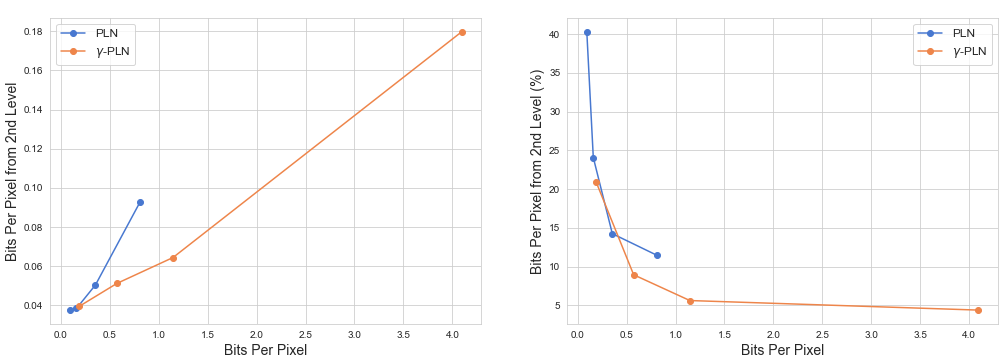
\includegraphics[width=\textwidth]{kodim05_side_info.png}
  \caption[Contribution of the second level to the rate, plotted against the
    actual rate.]{Contribution of the second level to the rate, plotted against the
    actual rate. \textbf{Left:} Contribution in BPP, \textbf{Right:}
    Contribution in percentages. We see that for lower bitrates there is more
    contribution from the second level and it quickly decreases for higher
    rates. It is also clear that on the same bitrates, the $\gamma$-PLN requires
    less contribution from the second level than regular PLN.}
  \label{fig:kodim05_side_info}
\end{figure}

\subsection{Compression Speed}
\par
Although not a focus of our project, we now briefly examine the encoding and
decoding speed of our method. We have plotted the compression ratios of our
models against the time it took them to encode / decode them using IS-GS in
Figure \ref{fig:kodim05_coding_time}. As increasing the reconstruction quality
leads to higher KL divergences between the latent posteriors and priors, both the
importance sampler and the greedy sampler will need to split up a higher total
KL. Thus, we expect the coding to become slower, and is precisely what we
observe, with seemingly approximately linear growth. We also see that encoding
consistently takes around 3 times as long as decoding. It is clear that our
method is not yet practical:
even the fastest case takes around a minute to encode and about 20 seconds to
decode, which very far away for real-time applications for now. The precise
values are reported in Table \ref{tab:kodim05_coding_time}.
\begin{figure}
  \centering
  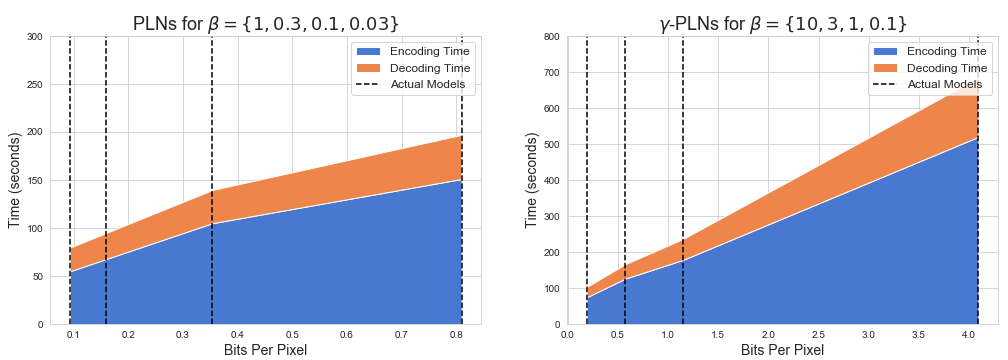
\includegraphics[width=\textwidth]{kodim05_coding_time.png}
  \caption[Coding times of models plotted against their rates.]
  {Coding times of models plotted against their rates. \textbf{Left:}
    Regular PLNs. \textbf{Right:} $\gamma$-PLNs. The striped lines indicate
    the concrete positions of our models in the rate line. While it seems
    that there is a
    linear relationship between rate and coding time, we do not have enough
    data points to conclude this.}
  \label{fig:kodim05_coding_time}
\end{figure}

\begin{table}[]
  \centering
  \begin{tabular}{|r||c|c|c|c||c|c|c|c|}
    \hline
    & \multicolumn{4}{c||}{\textbf{PLNs}} & \multicolumn{4}{c|}{\textbf{$\gamma$-PLNs}} \\
    \hline 
    $\beta$ & 1 & 0.3 & 0.1 & 0.03 & 10 & 3 & 1 & 0.1 \\ 
    \hline\hline
    Encoding Time (s) & 55.91 & 64.95 & 98.85 & 145.38 & 71.40 & 120.54 & 172.34 & 452.49 \\
    \hline
    Decoding Time (s) & 24.85 & 26.61 & 33.34 & 44.85 & 27.81 & 38.87 & 54.86 & 140.52 \\
    \hline
  \end{tabular}
  \caption{Compression times of our models for various compression rates.}
  \label{tab:kodim05_coding_time}
\end{table}